\documentclass[a4paper,10pt]{report}
\usepackage[T1]{fontenc}
\usepackage{titlesec}
\usepackage{graphicx}
\usepackage{svg}
\usepackage{amsmath}
\usepackage{amsthm}
\usepackage{fancyvrb}
\usepackage[english]{babel}
\usepackage{csquotes}
\usepackage{hyperref}
\hypersetup{
   colorlinks=true,
   linkcolor=blue,
   urlcolor=cyan
}
\usepackage{tikz}
\usepackage{amssymb}
\usepackage[sc]{mathpazo}
\linespread{1.05}
\usepackage{microtype}
\usepackage{breqn}
\usepackage{caption}
\usepackage{subcaption}
\usepackage{minted}
\setminted{
   numberblanklines=false, 
   mathescape, 
   texcomments, 
   autogobble, 
   breakanywhere, 
   breakautoindent, 
   breaklines,
   frame=none
}
\setminted[python]{python3}
\usepackage[
   backend=biber,%
   bibencoding=utf8,%
   language=english,%
   style=numeric-comp,%
   sorting=nyt,%
   maxbibnames=10,%
   natbib=true%
]{biblatex}
\addbibresource{references.bib}
\usepackage{blkarray}
\usepackage{siunitx}
\graphicspath{ {./img/} }

% Set TOC depth and sections numbering
\setcounter{tocdepth}{3}
\setcounter{secnumdepth}{3}

% Remove chapters head
\titleformat{\chapter}[display]
  {\normalfont\bfseries}{}{0pt}{\Large}

% Make quotes italic 
\renewcommand{\mkbegdispquote}[2]{\itshape}


\begin{document}
\frenchspacing

% First page
\title{
	{{\large{\textsc{Alma Mater Studiorum $\cdot$ University of Bologna}}}}
	\rule{\textwidth}{0.4pt}\vspace{3mm}
	\textbf{Flatland Challenge} 
	\begin{figure}[!htb]
		\centering
		\includesvg[width = 200pt]{flatland-logo}
	\end{figure} \\
	Deep learning course final project
}

\author{Leonardo Calbi (\href{mailto:leonardo.calbi@studio.unibo.it}{leonardo.calbi@studio.unibo.it}) \\ Alessio Falai (\href{mailto:alessio.falai@studio.unibo.it}{alessio.falai@studio.unibo.it})}
\date{\today}
\maketitle
\newpage
\tableofcontents
\listoffigures
\newpage


\chapter*{Foreword}
The Flatland challenge is a competition organized by AIcrowd \cite{aicrowd} with the help of SBB (Swiss Federal Railways) to foster innovation with what regards the scheduling of trains trajectories in a railway environment. 

As reported on the official challenge website, SBB operates the densest mixed railway traffic in the world. It maintains and operates the biggest railway infrastructure in Switzerland. Today, there are more than $\num{10000}$ trains running each day, being routed over $\num{13000}$ switches and controlled by more than $\num{32000}$ signals. 

The Flatland challenge aims to address the vehicle rescheduling problem by providing a simplistic grid world environment and allowing for diverse solution approaches. In particular, the first edition of the challenge was hosted during 2019 and the submitted solutions were mainly based on OR (Operation Research) methodologies, while the second edition of the competition, i.e. the NeurIPS 2020 edition, had the goal of favoring the implementation of RL (Reinforcement Learning) based solutions.  


\chapter{Introduction}
At the core of this challenge lies the general vehicle re-scheduling problem (VRSP) proposed \citeauthor{vrsp} in \citeyear{vrsp} \cite{vrsp}:
\begin{displayquote}
	The vehicle rescheduling problem (VRSP) arises when a previously assigned trip is disrupted. A traffic accident, a medical emergency, or a breakdown of a vehicle are examples of possible disruptions that demand the rescheduling of vehicle trips. The VRSP can be approached as a dynamic version of the classical vehicle scheduling problem (VSP) where assignments are generated dynamically.
\end{displayquote}

The problem is formulated as a 2D grid environment with restricted transitions between neighboring cells to represent railway networks. On the 2D grid, multiple agents with different objectives must collaborate to maximize the global reward.

The overall goal is to make all agents (trains) arrive at their target destination with a minimal travel time. In other words, we want to minimize the time steps (or wait time) that it takes for each agent in the group to reach its destination.


\chapter{Background}
As already pointed out, the Flatland environment is represented as a 2D grid and each cell can be one of many different types. The different types of cells can belong to the following categories: \texttt{rail} and \texttt{empty}.

The \texttt{rail} cells are the most intricated of the two, in that there exists different types of them. In particular, figure \ref{fig:rail-cells} shows examples of possible \texttt{rail} cells that can be used to build up a railway environment in Flatland. Other than the ones shown in figure \ref{fig:rail-cells} there are also diamond crossings (i.e. two orthogonal straight rails crossing each other), single slip switches (i.e. the same as double slip switches but with a single choice) and symmetrical switches (which are special kinds of switches that bifurcate to a left and right branch). Moreover, every \texttt{rail} cell can be rotated by $90^{\circ}$ and mirrored along both axis, to allow more combinations between them to be made, in order to guarantee a great degree of diversity between different railways.

\begin{figure}[h]
	\centering
	\captionsetup[subfigure]{justification=centering}
	\begin{subfigure}[t]{.25\linewidth}
		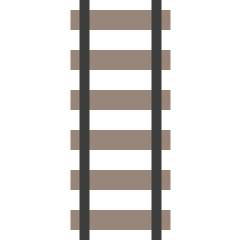
\includegraphics[width=\textwidth]{straight-rail.png}
		\caption{Straight}
		\label{fig:rail-cell-straight}
	\end{subfigure}%
    ~
	\begin{subfigure}[t]{.25\linewidth}
		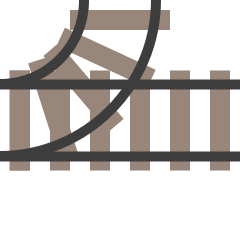
\includegraphics[width=\textwidth]{simple-switch-rail.png}
		\caption{Simple switch}
		\label{fig:rail-cell-simple}
	\end{subfigure}%
	~ 
	\begin{subfigure}[t]{.25\linewidth}
		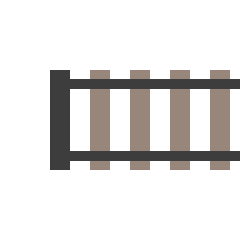
\includegraphics[width=\textwidth]{deadend-rail.png}
		\caption{Deadend}
		\label{fig:rail-cell-deadend}
	\end{subfigure}%
	~
	\begin{subfigure}[t]{.25\linewidth}
		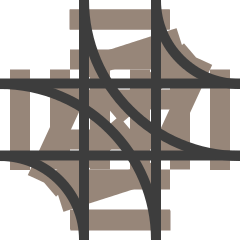
\includegraphics[width=\textwidth]{double-slip-rail.png}
		\caption{Double slip switch}
		\label{fig:rail-cell-double}
	\end{subfigure}%
    
	\caption{Different \texttt{rail} cell types}
	\label{fig:rail-cells}
\end{figure}

Moreover, \texttt{rail} cells can be occupied by the following entities (the ones shown in figure \ref{fig:agent-target}):
\begin{itemize}
	\item Agent: one \texttt{rail} cell can be seen as a resource with availability equal to one, so that in each time step only one agent can occupy it
	\item Target: they represent the destination of one or more agents (different agents could have the same target) and the number of possible targets present in the environment is clearly limited by the number of agents
\end{itemize}

\begin{figure}[h]
	\centering
	\captionsetup[subfigure]{justification=centering}
	\begin{subfigure}[t]{.25\linewidth}
		
\includegraphics[width=\textwidth]{agent.png}
		\caption{Agent example}
		\label{fig:agent}
	\end{subfigure}%
    ~
	\begin{subfigure}[t]{.25\linewidth}
		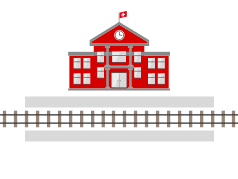
\includegraphics[width=\textwidth]{target.png}
		\caption{Target example}
		\label{fig:target}
	\end{subfigure}%
	\caption{Agents and targets}
	\label{fig:agent-target}
\end{figure}

An important fact about the different types of \texttt{rail} cells is that only switches require an agent to make a choice. In Flatland (like in reality) a maximum of two options is available. There does not exist a switch with three or more options.

Finally, every cell that is not \texttt{rail} is \texttt{empty} and neither targets nor agents can fill it up. As shown in figure \ref{fig:env-example}, it is interesting to notice that Flatland is a very sparse environment, meaning that there are a lot more \texttt{empty} cells than \texttt{rail} ones: because of this, representing the environment as a simple dense matrix could lead to overheads and efficiency issues, especially when dealing with relatively big environments.

In the end, the only cell types that we care about are the \texttt{rail} ones: the \texttt{empty} ones are useful only for visualization purposes. Because of this, we could think of representing the environment as a sparse matrix or as a graph containing only \texttt{rail} cells or a subset of them (we will address this issue in chapter ??????????????????).

\begin{figure}[h]
	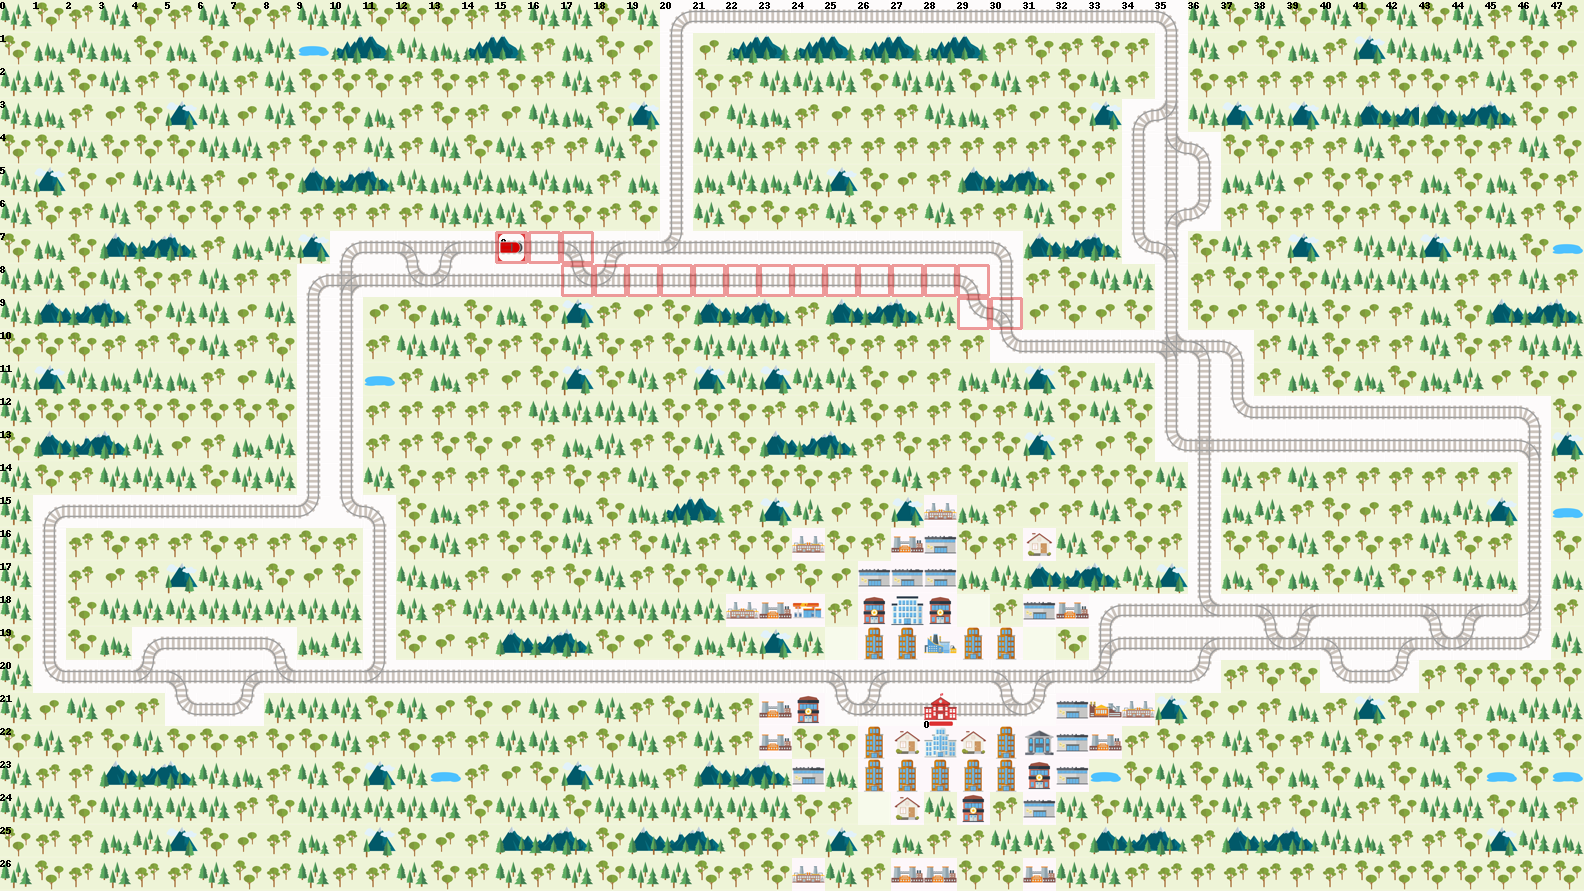
\includegraphics[width=\textwidth]{env.png}
	\caption{An example of a railway environment}
	\label{fig:env-example}
\end{figure}

An agent in the Flatland environment is a train that starts from a random \texttt{rail} cell in the map and has to arrive to its assigned \texttt{target} cell in the minimum number of steps. To do so, the agent can only occupy \texttt{rail} cells. 

To move from a cell to another one the agent has to make a choice and, depending on the cell type that they are on and on the connections between cells, an agent can transition from cell $i$, when looking towards direction $d_i$, to cell $j$, looking towards direction $d_j$, if and only if $T_i(d_i, d_j)=1$, where $T_i$ is the transition matrix associated to cell $i$, s.t. $T_i(d_i, d_j)=0$ means that the transition from cell $i$, direction $d_i$ to cell $j$, direction $d_j$ is forbidden (likewise $T_i(d_i, d_j)=1$ means that the transition is allowed). Directions $d_*$ are represented as the $4$ cardinal directions, i.e. North, East, South and West (N, E, S, W), so that each transition matrix $T_*$ can be characterized as a $4\times4$ binary matrix. For example, a deadend cell like the one reported in figure \ref{fig:rail-cell-deadend} would have a transition matrix like the one shown in figure \ref{fig:rail-cell-bitmap}.

\begin{figure}[h]
	\noindent\begin{minipage}{.5\linewidth}
		\begin{equation*}
			\begin{blockarray}{ccccc}
				& N & E & S & W \\
				\begin{block}{c(cccc)}
				N & 0 & 0 & 0 & 0 \\
				E & 0 & 0 & 0 & \mathbf{1} \\
				S & 0 & 0 & 0 & 0 \\
				W & 0 & 0 & 0 & 0 \\
				\end{block}
			\end{blockarray}
		\end{equation*}
	\end{minipage}%
	$\xrightarrow[\text{bitmap}]{\text{to}}$
	\begin{minipage}{.5\linewidth}
		\begin{equation*}
			0000 \; 000\mathbf{1} \; 0000 \; 0000
		\end{equation*}
	\end{minipage}
	\caption{Example of a \texttt{rail} cell transition matrix and bitmap}
	\label{fig:rail-cell-bitmap}
\end{figure}

As we can observe, only one entry in the matrix has value $1$, meaning that only one transition is possible, i.e. the one s.t. the agent enters heading East and exits heading West. 

In the Flatland library, a transition matrix is represented by a bitmap, which can be seen as a linearization by rows of the reported matrix (the mapping between the transition matrix of the deadend cell \ref{fig:rail-cell-deadend} and its bitmap is again shown in figure \ref{fig:rail-cell-bitmap}). In this way, by simply counting the number of true values in the bitmap, we can understand the type of \texttt{rail} cell that we are examining (e.g. only one true value indicates a deadend, while exactly two true values indicate a straight rail). 

Flatland has a discrete action space, meaning that only $5$ possibilities have to be considered at each transition. In particular, Flatland uses the following convention:
\begin{enumerate}
	\item \texttt{MOVE_FORWARD}: the agent maintains the current movement direction, if possible (i.e. if it was heading North, it will continue heading North)
	\item \texttt{MOVE_LEFT}: if the agent is at a switch with a transition to its left, the agent will choose the left path, otherwise the action has no effect
	\item \texttt{MOVE_RIGHT}: if the agent is at a switch with a transition to its right, the agent will choose the right path, otherwise the action has no effect
	\item \texttt{STOP_MOVING}: the agent remains in the same cell
	\item \texttt{DO_NOTHING}: the agent performs the same action as the last time step
\end{enumerate}

Usually, only a handful of the reported actions can be perfomed on a given cell, meaning that most of the times the actual number of choices is much less than $5$ (we will address this issue in chapter ??????????????????).

\chapter{Environment}
\section{Railway encoding}
\section{Observations}
\subsection{Tree}
\subsection{Binary tree}
\section{Predictions}
\subsection{Shortest path}
\section{Choices}
\section{Rewards shaping}

\chapter{Policy}
\section{Action masking}
\section{Action selection}
\subsection{$\epsilon$-greedy}
\subsection{Boltzmann}
\section{Replay buffers}
\subsection{Uniform}
\subsection{Prioritized}

\chapter{DQN}
\section{Architectures}
\subsection{Vanilla}
\subsection{Double}
\subsection{Dueling}
\section{Bellman equation}
\subsection{Max}
\subsection{Softmax}

\chapter{GNN}

\chapter{Results}



\chapter{Conclusions}

\printbibliography

\end{document}
